\documentclass{article}
\usepackage[utf8]{inputenc}
\usepackage[spanish]{babel}
\usepackage{graphicx}
\usepackage{anysize}
\usepackage{fancyhdr} 
\usepackage[export]{adjustbox}
\usepackage{titlesec}
\usepackage{enumitem}
\usepackage{listings}
\usepackage{xcolor}

% \usepackage{hyperref}
% \usepackage{float}
% \usepackage{tabu}

% Izquierda, derecha, arriba, abajo
\marginsize{2cm}{2cm}{1.2cm}{1.5cm} 
\renewcommand{\familydefault}{\sfdefault}
\decimalpoint%

\graphicspath{{assets/}}

\setlength{\parindent}{0in}
\titleformat*{\section}{\large\bfseries}

% Para insert código
\definecolor{codegreen}{rgb}{0,0.6,0}
\definecolor{codegray}{rgb}{0.5,0.5,0.5}
\definecolor{codepurple}{rgb}{0.58,0,0.82}
\definecolor{backcolour}{rgb}{1,1,1}

\usepackage{textcomp}
\lstset{upquote=true}
\lstdefinestyle{mystyle}{
    backgroundcolor=\color{backcolour},   
    commentstyle=\color{codegreen},
    keywordstyle=\color{magenta},
    numberstyle=\tiny\color{codegray},
    stringstyle=\color{codepurple},
    basicstyle=\ttfamily\footnotesize,
    breakatwhitespace=false,         
    breaklines=true,                 
    captionpos=b,                    
    keepspaces=true,                 
    % numbers=left,                    
    % numbersep=5pt,                  
    showspaces=false,                
    showstringspaces=false,
    showtabs=false,                  
    tabsize=2
}

\lstset{style=mystyle}

\newcommand{\materia}{BDA}
\newcommand{\clave}{2929}
\newcommand{\profesor}{Ing. Rodriguez Campos \textsc{Jorge Alberto}}
\newcommand{\grupo}{1}
\newcommand{\semestre}{2021-1}

\newcommand{\alumno}{Francisco Pablo \textsc{Rodrigo}}

\newcommand{\actividad}{Tema 02 \\ Ejercicio práctico 02}
\newcommand{\titulo}{Configuraciones previas a la creación de una base de datos}

\newcommand{\fechaEntrega}{15 de octubre de 2020}

%%%%%%%%%%%%%%%%%%%% ENCABEZADO %%%%%%%%%%%%%%%%%%%%%%%%%%%%
\pagestyle{fancy}
\fancyhf{}
\renewcommand{\headrulewidth}{0pt}
\fancyhead[R]{% Left header
    \begin{tabular}{l}
        \materia \\ 
        \actividad%
    \end{tabular}
    \,% Space
    \rule[-1.75\baselineskip]{0pt}{0pt}
    % Strut to ensure a 1/4 \baselineskip between image and header rule
    
\includegraphics[height=3\baselineskip,valign=c]{unam}
}
\setlength{\headsep}{0.3in}


\begin{document}
%%%%%%%%%%%%%%%%%%% DATOS PORTADA %%%%%%%%%%%%%%%%%%%%%%%%
\thispagestyle{empty}
\begin{minipage}[t][5cm][t]{0.2\linewidth}
    
\includegraphics[width=2.5cm]{unam.jpg}
    \vspace{10cm}

    
\includegraphics[width=2.5cm]{fiblack}
\end{minipage}
\begin{minipage}[t]{0.7\linewidth}
    \vspace{-2.5cm}
    \LARGE{\textbf{Universidad Nacional Autónoma de México}}\\
    \Large{\textbf{Facultad de Ingeniería}} \\

    \large{\semestre}\\[2cm]

    \large{\textbf{\materia (\clave)}}\\
    \large{\textbf{Gpo: 1}}\\[5mm]
    \large{\textbf{Profesor:} \profesor}\\ [1.5cm]
    \begin{center}
        \LARGE{\textbf{\actividad}}\\
        \LARGE{\textbf{\titulo}}\\
    \end{center}

    \vspace{3.3cm}

    \large{\textbf{Alumno:} \alumno} \\[1.5cm]

    \begin{flushright}
        \fechaEntrega%
    \end{flushright}
\end{minipage}

\newpage
%%%%%%%%%%%%%%%%%%% CONTENIDO %%%%%%%%%%%%%%%%%%%%%%%%

\section*{Objetivos}
Comprender y poner en práctica el proceso básico para realizar todas las 
configuraciones necesarias para crear una base de datos a través de la
instrucción \texttt{create database}.

\section*{C1. Código del script \texttt{s-01-crea-loop-devices.sh}}

\lstinputlisting[language=Bash]
{tema02-ej-prac-02-codigo/s-01-crea-loop-devices.sh}

\newpage
\section*{C2. Código del script \texttt{s-02-crea-pwd-param.sh}}

\lstinputlisting[language=Bash, lastline=34]
{tema02-ej-prac-02-codigo/s-02-crea-pwd-param.sh}

\section*{C3. Salida del validador.}

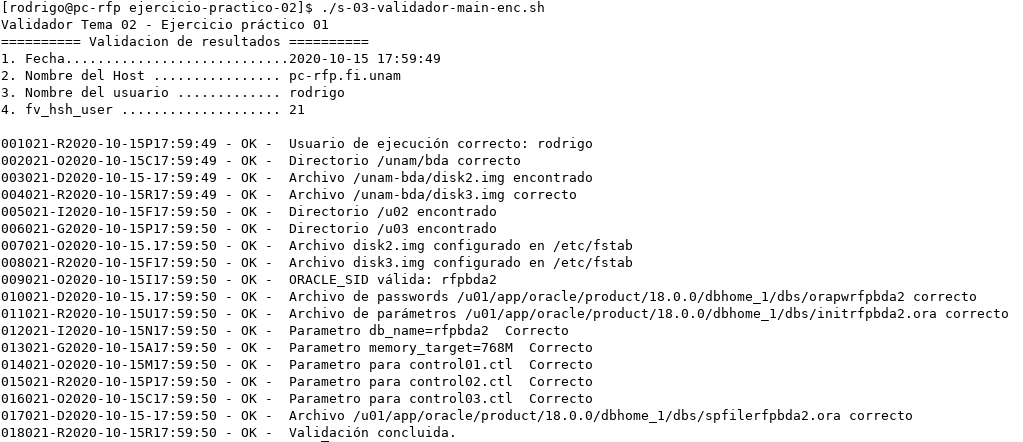
\includegraphics[width=\linewidth]{tema02-ej-prac-02-validador}

\section*{C5. Comentarios y conclusiones}

Automatizar la configuración previa a la creación de la base de datos nos 
permitirá ahorrarnos tiempo y si algo sale mal basta con ejecutar nuevamente
el script. De hecho podríamos verlo como nuestro \textit{save point}.
Entre más automaticemos menos nos tardaremos a la hora de hacer pruebas
con la creación de la bases de datos y todos sus artefactos. De ahí la 
importancia de crear scripts robustos y bien hechos.

\renewcommand\refname{Bibliografía y referencias}
\begin{thebibliography}{99}
    \bibitem{burleson} Burleson Consulting. \textit{Oracle tips } en 
    \texttt{http://www.dba-oracle.com/oracle\_news/}
    \bibitem{shellscript} Steve Parker. \textit{Changing to Uppercase or 
    Lowercase} en \texttt{https://www.shellscript.sh/tips/case/} 
\end{thebibliography}

\end{document}
